%% Compilar usando PDFLaTeX
\documentclass[10pt,a4paper,notitlepage]{article}
\usepackage[spanish]{babel}
\usepackage[utf8]{inputenc}
\usepackage[T1]{fontenc}

\usepackage{amsmath}
\usepackage{amsthm}
\usepackage{amsfonts}
\usepackage{amssymb}
\usepackage{algorithm}
\usepackage{algpseudocode}
\usepackage{graphicx}

\newtheorem{deftn}{Definición}
\newtheorem{defthm}{Teorema}

\author{Julián Bayardo}
\title{Resumen de Inducción/Recursión}
\begin{document}
\section{Mejorando la performance de una recursión}

\subsection{Inmersión de Rango / Generalización de Funciones}

Una forma de hacer que una recursión que depende de $k$ resultados anteriores es agregar información adicional sobre los $k$ pasos anteriores en el retorno de la función. Por ejemplo, si tenemos una recursión

$$b_n = f(b_{n-1}, b_{n-2}, ..., b_{n-k})$$

Podemos transformarla en una recursión de la forma

$$c_n = \langle f(\pi_1(c_{n-1}), \pi_2(c_{n-1}), ..., \pi_k(c_{n-1})), \pi_1(c_{n-1}), \pi_2(c_{n-1}), ..., \pi_{k-1}(c_{n-1}) \rangle$$

Observemos que en esta última recursión sólo hace falta calcular $c_{n-1}$ una vez, y luego es simplemente tomar las componentes. La ventaja es que pasamos de tener un árbol de recursión de esta forma:

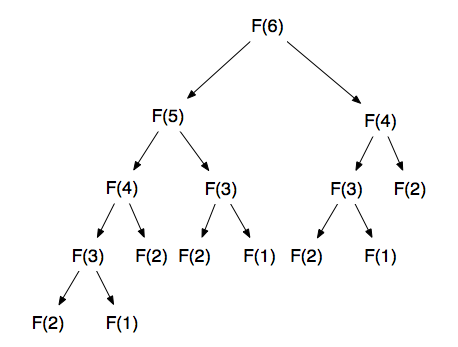
\includegraphics[width=0.8\textwidth]{Fib_Rec_Tree.png}

A tener una lista enlazada, donde $c_n$ depende unicamente de $c_{n-1}$. Utilizando esta misma idea (la de pasar los pasos anteriores de una recursión) podemos también combinar recursiones en una sola, poniendo los resultados parciales de la recursión dentro de una tupla, que es el resultado final. Observemos, aparte, que no necesariamente la recursión tiene que depender sequencialmente de $k$ casos anteriores, se puede aplicar este mismo método a recursiones cuyo cómputo utilice casos fragmentados.

\subsection{Inmersión de Dominio}

La idea es muy similar a inmersión de rango: en lugar de pasar los resultados parciales en una tupla, e ir computando el resultado actual bottom-up, pasamos los resultados que van a necesitar los casos más pequeños de manera top-down.

\subsection{Folding/Unfolding}

En folding/unfolding, intentamos obtener una recursión más veloz a través de reducir un poco la expresión original de nuestra función utilizando manipulación simbólica. La derivación del algorítmo de exponenciación rápida sobre monoides es un caso canónico.

\subsection{Memoization}

En el caso de recursiones que podrían ser llamadas muchas veces, son relativamente caras de llamar, y no dependen del estado externo de alguna estructura, una técnica muy común es la utilización de una caché para evitar recomputar datos. Un ejemplo factible es, por ejemplo, si sabemos que se va a computar Fibonacci muchas veces, podemos utilizar un arreglo para guardar los resultados parciales, en cuyo caso lo único que tendríamos que hacer es buscar si el valor ya fue computado, y si no lo fue computarlo y guardarlo en el arreglo.

%% Falta: cambio de orden de evaluación, evaluación parcial/currificación

\section{Eliminación de la recursión}

\subsection{Pros y contras de la recursión}

La utilización de recursión, si bien facilita ampliamente la comprensión de muchos algorítmos que tal vez son más difíciles de comprender en sus versiones recursivas (como el cómputo de altura de un árbol, búsqueda binaria sobre un arreglo, etcétera) y facilita la lectura del código, así como el proceso de eliminación de bugs, tiene varias desventajas respecto de sus contrapartes iterativas en la práctica, fundamentalmente por la forma en la que están diseñadas las computadoras.

En primer lugar, uno de los mayores problemas de la recursión es que cada llamada a una función requiere utilizar espacio en el stack para poner los argumentos de la misma. El espacio de stack acotado, mucho más acotado que la memoria de la máquina, por lo que si la recursión es muy profunda (es decir, el árbol de recursión tiene muchos nodos) el programa podría incurrir en un stack overflow, provocando que el sistema operativo mate el proceso.

En segundo lugar, perdemos la noción de estado implícita. Nótese que si uno necesitase mantener información extra a lo largo de la recursión (como un contador), las alternativas para poder utilizarlo involucran hacer inmersión de rango o de dominio. En los lenguajes imperativos, otra alternativa es utilizar una variable global (de cualquier forma, la utilización de variables globales es una práctica que suele evitarse por motivos de diseño).

En último lugar, suele ser difícil frenar una función recursiva por la mitad en caso de errores. Usualmente hacer esto requiere un tipo de mecanismo más o menos sofisticado para poder avisar a los niveles superiores del árbol de recursión que hubo un error más abajo (véase Maybe en Haskell, y excepciones más en general).

\subsection{Eliminación de la recursión}

Si bien podemos expresar las mismas funciones utilizando recursión que utilizando iteración, hay ciertos tipos de algorítmos recursivos que permiten ser convertidos a sus contrapartes iterativas automáticamente. En principio, dada cualquier función recursiva uno podría simular el stack con una estructura propia en el lenguaje de programación a elección, y así convertir las llamadas usuales a una función recursiva en una operación sobre nuestra estructura. Si bien esto es una posibilidad, es una forma demasiado complicada de acercarse al problema, y que probablemente no funcione bien.

%%%%%%%%%%%%%%%% JUSTIFICAR

Analizando casos particulares, las funciones recursivas lineales finales/a cola, es decir, aquellas con una única llamada recursiva que ocurre como último paso de la función, pueden ser automáticamente modificadas para ser iterativas. Por ejemplo, una función recursiva lineal final podría ser similar a:

\begin{algorithm}
\caption{Esqueleto y conversión de una función recursiva lineal final}\label{elimRecLinFinal1}
\begin{algorithmic}[1]
\Procedure{Función}{Parámetros}
\If {CasoBase(Parámetros)}
	\State \Return Valor
\Else
	\State \Return Función(Achicar(Parámetros))
\EndIf
\EndProcedure
\\
\Procedure{Convertida}{Parámetros}
\While {!CasoBase(Parámetros)}
	\State Parámetros $\gets$ Achicar(Parámetros)
\EndWhile
\State ...
\State \Return ValorFinal
\EndProcedure
\end{algorithmic}
\end{algorithm}

Otro caso particular son las funciones recusivas lineales que no son finales, es decir, con una única llamada recursiva pero no necesariamente con esta como último paso de la función. En estos casos, utilizando la técnica de inmersión de dominio podemos convertir la recursión en final automáticamente. El último caso en el cual podemos hacer eliminación de la recursión automáticamente es en el caso de las funciones recursivas no lineales múltiples, y las no lineales anidadas.

En particular, las no lineales múltiples pueden ser convertidas en no lineales anidadas a través de hacer inmersión de dominio, agregando un parámetro de acumulación que guarda los resultados parciales de las llamadas recursivas.

%% EJEMPLOSSSSSSSSSSSSSSSSSSSSSSSSSS

En el caso de las no lineales anidadas la técnica involucra utilizar una pila para guardar los resultados parciales, de esta forma convirtiendola en una función recursiva final, que por otro lado ya sabemos como convertir en iterativa.

\section{Inducción sobre TADs}

Te pedía básicamente plantear el esquema de inducción estructural para un TAD genérico, y justificar que se puede usar inducción en los TADs.
Se puede hacer inducción sobre los reales? Y sobre el TAD racionales? Justifique.

\subsection{Esquema de inducción}

Dada una proposición $P$ sobre un TAD T, si tomamos a $g_1, ..., g_k$ como los generadores del TAD que no toman ninguna instancia de argumento, a $g_{k+1}, ..., g_n$ como los generadores que sí toman una instancia previa, entonces tenemos el esquema de inducción sobre T

$$(\bigwedge_{i=1}^k P(g_i) \wedge \bigwedge_{i=k+1}^n (\forall t : T) (P(t) \implies P(g_i(t)))) \implies (\forall t : T) P(t)$$

Observemos que esta fórmula no contempla generadores que reciban parámetros de otro tipo. En estos casos, lo único que hace falta es agregar una cuantificación universal por cada parámetro de otro tipo en los lugares adecuados. Suponiendo que $T_1, ..., T_n$ es el tipo de cada argumento que recibe cada generador, el esquema de inducción sería:

$$(\bigwedge_{i=1}^k [(\forall a : T_i) P(g_i(a))] \wedge \bigwedge_{i=k+1}^n (\forall t : T) (P(t) \implies ((\forall a : T_i) P(g_i(t, a))))) \implies (\forall t : T) P(t)$$

\subsection{Fundamentos teóricos}

\begin{deftn}
Sea $S$ un conjunto, $\star$ una relación binaria sobre $S$. Decimos entonces que $\star$ es:

\begin{itemize}
\item Reflexiva $\iff (\forall a \in S) (a \star a)$
\item Simétrica $\iff (\forall a, b \in S) (a \star b \implies b \star a)$
\item Transitiva $\iff (\forall a, b, c \in S) (a \star b \wedge b \star c \implies a \star c)$
\item Antisimétrica $\iff (\forall a, b \in S) (a \star b \wedge b \star a \implies a = b)$
\item Total $\iff (\forall a, b \in S) (a \star b \vee b \star a)$
\end{itemize}
\end{deftn}

\begin{deftn}
Denominamos un orden parcial (poset) a un conjunto $S$ junto con una relación binaria $\prec$ definida sobre $S$ tal que $\prec$ es reflexiva, antisimétrica, y transitiva
\end{deftn}

\begin{deftn}
En el caso en que $\prec$ es transitiva, antisimétrica y total, decimos que $\prec$ es un orden total.
\end{deftn}

\begin{deftn}
Si tenemos $\prec$ un orden total sobre $S$ y para todo subconjunto no vacio de $S$ hay un elemento mínimo, decimos que $\prec$ es un buen orden sobre $S$.
\end{deftn}

\begin{defthm}
Principio de inducción bien fundada: si $\prec$ define un buen orden sobre $S$, $P$ es un predicado sobre $S$, y

\begin{itemize}
\item P vale para todos los elementos mínimos de S de acuerdo a $\prec$.
\item $(\forall a \in S) [(\forall b \in S) (b \prec a \implies P(a))]$
\end{itemize}

Entonces, $(\forall a \in S) P(a)$
\end{defthm}

\begin{proof}[Principio de inducción bien fundada]
Por el contrarreciproco, supongamos que $\exists a \in S : \neg P(a)$, para demostrar la validez del teorema, lo que necesitamos es mostrar que $P$ no vale para todos los elementos mínimos de $S$, o que existe un elemento $a$ de S tal que existe un $b$ en S y $\neg(b \prec a \implies P(a))$

Sabemos que el conjunto $\{x : x \in S \wedge \neg P(x)\}$ es no vacio, y tiene un elemento mínimo $m$ determinado por $\prec$ porque $\prec$ define un buen orden sobre $S$. Si $m$ es un elemento mínimo de $S$, entonces no hay nada más que hacer, porque tendríamos que la primera condición es falsa. En el caso contrario, existen elementos de $S$ que son menores a $m$, pero observemos que todos esos elementos menores a $m$ sí cumplen $P$ (porque sino serían m), pero la segunda condición dice que entonces debería valor $P(m)$. Contradicción.
\end{proof}

Solo falta ver por qué existe un orden bien fundado sobre TADs. Notemos, primero, que las instancias de un TAD son numerables: todas las instancias de un TAD son generadas a través de un cantidad finita de aplicaciones de los generadores sobre una instancia inicial. Por lo tanto, existe una biyección con los naturales.

\end{document}